

%% AAPT Physics Bowl Exams Questions
%%----------------------------------------


%% this section contains 34 problems


%% PhysicsBowl 2015
%%----------------------------------------
\element{aapt}{ %% Bowl-A5
\begin{question}{bowl-2015-q03}
    Which one of the following quantities is not a vector quantity?
    \begin{multicols}{2}
    \begin{choices}
      \correctchoice{Average speed}
        \wrongchoice{Average velocity}
        \wrongchoice{Linear momentum}
        \wrongchoice{Acceleration}
        \wrongchoice{Average force}
    \end{choices}
    \end{multicols}
\end{question}
}

\element{aapt}{ %% Bowl-A5
\begin{question}{bowl-2015-q12}
    A box of mass \SI{12.0}{\kilo\gram} is being pushed
        to the right across a horizontal surface.
    When the box has \SI{12.0}{\joule} of kinetic energy,
        a \SI{12.0}{\newton} net force acts on it.
    Which one of the following choices best represents the
        magnitude of the linear momentum of the box at this instant?
    \begin{multicols}{2}
    \begin{choices}
        \wrongchoice{\SI{6.00}{\kilo\gram\meter\per\second}}
        \wrongchoice{\SI{8.50}{\kilo\gram\meter\per\second}}
        \wrongchoice{\SI{12.0}{\kilo\gram\meter\per\second}}
      \correctchoice{\SI{17.0}{\kilo\gram\meter\per\second}}
        \wrongchoice{\SI{24.0}{\kilo\gram\meter\per\second}}
    \end{choices}
    \end{multicols}
\end{question}
}

\newcommand{\BowlTwentyFifteenQTwentySeven}{
\begin{tikzpicture}
    \begin{axis}[
        axis y line=left,
        axis x line=bottom,
        axis line style={->},
        xlabel={time},
        x unit=\si{\milli\second},
        xtick={0,1,2,3},
        ylabel={force},
        y unit=\si{\kilo\newton},
        ytick={0,5,10},
        grid=major,
        xmin=0,xmax=3,
        ymin=0,ymax=10,
        width=0.95\columnwidth,
        height=0.50\columnwidth,
    ]
    \addplot[line width=1pt,mark=\empty] plot coordinates {(0,0) (1,10) (3,0) };
    \end{axis}
\end{tikzpicture}
}

\element{aapt}{ %% Bowl-A5
\begin{question}{bowl-2015-q27}
    %Questions 27 – 28 deal with the following information:
    On a frictionless horizontal surface,
        two bodies make a head-on collision and stick together.
    Body 1 has a mass of \SI{3.50}{\kilo\gram} and initially moves
        to the right with speed \SI{7.0}{\meter\per\second}.
    Body 2 initially is at rest.
    A graph of the force exerted onto Body 2 from Body 1 during the collision is shown.
    \begin{center}
        \BowlTwentyFifteenQTwentySeven
    \end{center}
    What is the mass of Body 2?
    \begin{multicols}{3}
    \begin{choices}
        \wrongchoice{\SI{2.81}{\kilo\gram}}
        \wrongchoice{\SI{3.50}{\kilo\gram}}
        \wrongchoice{\SI{4.59}{\kilo\gram}}
      \correctchoice{\SI{5.53}{\kilo\gram}}
        \wrongchoice{\SI{7.50}{\kilo\gram}}
    \end{choices}
    \end{multicols}
\end{question}
}

\element{aapt}{ %% Bowl-A5
\begin{question}{bowl-2015-q28}
    %Questions 27 – 28 deal with the following information:
    On a frictionless horizontal surface,
        two bodies make a head-on collision and stick together.
    Body 1 has a mass of \SI{3.50}{\kilo\gram} and initially moves
        to the right with speed \SI{7.0}{\meter\per\second}.
    Body 2 initially is at rest.
    A graph of the force exerted onto Body 2 from Body 1 during the collision is shown.
    \begin{center}
        \BowlTwentyFifteenQTwentySeven
    \end{center}
    How much kinetic energy was transformed to other kinds of energy from the collision?
    \begin{multicols}{3}
    \begin{choices}
        \wrongchoice{\SI{67.1}{\joule}}
      \correctchoice{\SI{52.6}{\joule}}
        \wrongchoice{\SI{42.9}{\joule}}
        \wrongchoice{\SI{38.2}{\joule}}
        \wrongchoice{\SI{30.0}{\joule}}
    \end{choices}
    \end{multicols}
\end{question}
}

\element{aapt}{ %% Bowl-A5
\begin{question}{bowl-2015-q43}
    An object of mass \SI{4.0}{\kilo\gram} has a total kinetic energy of
        \SI{100.0}{\joule} and an $x$-component of
        linear momentum equal to \SI{24.0}{\kilo\gram\meter\per\second}.
    The object is moving in the $x$-$y$ plane.
    What is the $y$-component of the object's linear momentum?
    \begin{multicols}{2}
    \begin{choices}
        \wrongchoice{\SI{8.00}{\kilo\gram\meter\per\second}}
      \correctchoice{\SI{15.0}{\kilo\gram\meter\per\second}}
        \wrongchoice{\SI{26.0}{\kilo\gram\meter\per\second}}
        \wrongchoice{\SI{32.0}{\kilo\gram\meter\per\second}}
        \wrongchoice{\SI{97.0}{\kilo\gram\meter\per\second}}
    \end{choices}
    \end{multicols}
\end{question}
}


%% PhysicsBowl 2014
%%----------------------------------------
\element{aapt}{ %% Bowl-A5
\begin{question}{bowl-2014-q15}
    Two objects $A$ and $B$, move in space and then collide.
    \begin{description}
        \item[Before collision:] Object $A$, of mass \SI{5.0}{\kilo\gram},
            moves to the right with a speed of \SI{25.0}{\meter\per\second}.
            Object $B$ of mass \SI{10.0}{\kilo\gram}, moves to the left
            with a speed of \SI{20.0}{\meter\per\second}.
        \item[After collision:] Object $A$ moves to the left with a speed
            of \SI{25.0}{\meter\per\second}.
    \end{description}
    What is the velocity of object $B$ after the collision?
    \begin{multicols}{2}
    \begin{choices}
        \wrongchoice{\SI{30.0}{\meter\per\second} to the right}
        \wrongchoice{\SI{20.0}{\meter\per\second} to the right}
        \wrongchoice{\SI{20.0}{\meter\per\second} to the left}
      \correctchoice{\SI{5.0}{\meter\per\second} to the right}
        \wrongchoice{\SI{5.0}{\meter\per\second} to the left}
    \end{choices}
    \end{multicols}
\end{question}
}


%% PhysicsBowl 2013
%%----------------------------------------
\element{aapt}{ %% Bowl-A5
\begin{question}{bowl-2013-q05}
    At an instant of time $t$, a point object of mass $M$ moves with velocity $\vec{V}$,
        has acceleration $\vec{A}$, and is at position $(x,y)$.
    In what direction must the linear momentum of the object be directed at this instant?
    \begin{choices}
      \correctchoice{Along the direction of the velocity of the mass.}
        \wrongchoice{Along the direction of the net force acting on the mass.}
        \wrongchoice{Along the direction of the vector from the origin $(0,0)$ to $(x,y)$.}
        \wrongchoice{Along the direction of the acceleration of the mass.}
        \wrongchoice{Along the direction perpendicular to the object's acceleration.}
    \end{choices}
\end{question}
}

\element{aapt}{ %% Bowl-A5
\begin{question}{bowl-2013-q42}
    An object of mass $12M$ is at rest when it suddenly explodes into 3 pieces with masses $3M$, $4M$, and $5M$.
    The piece of mass $3m$ moves with speed $V$ in the direction shown in the diagram.
    \begin{center}
    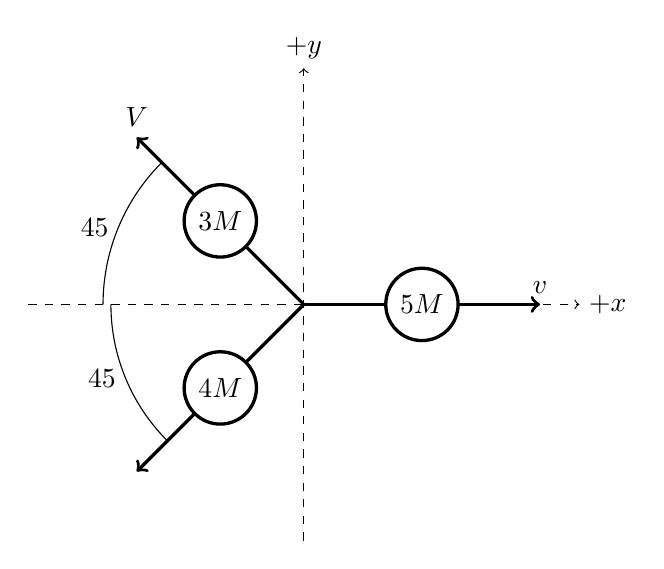
\begin{tikzpicture}
        \draw[dashed,->] (0,-3) -- (0,+3) node[anchor=south] {$+y$};
        \draw[dashed,->] (-3.5,0) -- (+3.5,0) node[anchor=west] {$+x$};
        %% First Mass
        \draw[very thick,->] (0,0) -- ++ (135:3)
            node[pos=1.0,anchor=south] {$V$}
            node[pos=0.5,draw,circle,fill=white,anchor=center] {$3M$};
        \draw (180:2.55) arc (180:135:2.55)
            node[pos=0.5,anchor=east] {\ang{45}};
        %% Second Mass
        \draw[very thick,->] (0,0) -- ++ (225:3)
            node[pos=0.5,draw,circle,fill=white,anchor=center] {$4M$};
        \draw (225:2.45) arc (225:180:2.45)
            node[pos=0.5,anchor=east] {\ang{45}};
        %% Third Mass
        \draw[very thick,->] (0,0) -- ++ (0:3)
            node[pos=1.0,anchor=south] {$v$}
            node[pos=0.5,draw,circle,fill=white,anchor=center] {$5M$};
    \end{tikzpicture}
    \end{center}
    What is the speed of the piece with mass $5M$ knowing it is moving directly to the right?
    \begin{multicols}{3}
    \begin{choices}
        \wrongchoice{$V$}
        \wrongchoice{$\dfrac{3\sqrt{2}}{20}V$}
      \correctchoice{$\dfrac{3\sqrt{2}}{5}V$}
        \wrongchoice{$\dfrac{3}{5\sqrt{2}}V$}
        \wrongchoice{$\dfrac{7}{5\sqrt{2}}V$}
    \end{choices}
    \end{multicols}
\end{question}
}

\element{aapt}{ %% Bowl-A5
\begin{question}{bowl-2013-q43}
    A small \SI{1.0}{\kilo\gram} mass is launched from the top of a cliff with speed $V$ at an angle of \ang{30} above the horizontal.
    When the mass reaches the ground, its velocity is directed at \ang{45} below the horizontal.
    Which one of the following choices is the magnitude of the total impulse that was imparted to the mass during its flight?
    Ignore air resistance.
    \begin{multicols}{2}
    \begin{choices}
      \correctchoice{$\dfrac{1}{2}\left(\sqrt{3}+1\right)V$}
        \wrongchoice{$\sqrt{\dfrac{3}{2}}\dfrac{\left(\sqrt{2}+1\right)}{2}V$}
        \wrongchoice{$\dfrac{1}{2}\left(\sqrt{3}-1\right)V$}
        \wrongchoice{$\dfrac{1}{2}\left(\sqrt{\dfrac{3}{2}}+1\right)V$}
        \wrongchoice{$\sqrt{\dfrac{3}{2}}\dfrac{\left(\sqrt{2}+1\right)}{\left(\sqrt{2}-1\right)}V$}
    \end{choices}
    \end{multicols}
\end{question}
}



%% PhysicsBowl 2012
%%----------------------------------------
\element{aapt}{ %% Bowl-A5
\begin{question}{bowl-2012-q12}
    Which one of the following quantities is a scalar quantity?
    \begin{multicols}{2}
    \begin{choices}
        \wrongchoice{Impulse}
        \wrongchoice{Linear Momentum}
        \wrongchoice{Acceleration}
      \correctchoice{Speed}
        \wrongchoice{Displacement}
    \end{choices}
    \end{multicols}
\end{question}
}

\element{aapt}{ %% Bowl-A5
\begin{question}{bowl-2012-q23}
    A collision of two blocks takes place along a
        horizontal surface without friction.
    A block with mass $M_1=\SI{3.00}{\kilo\gram}$ initially moves to the left with speed
        $V_1=\SI{5.00}{\meter\per\second}$ when its hits a block with mass
        $M_2=\SI{5.00}{\kilo\gram}$ initially moving to the right with speed
        $V_2=\SI{2.00}{\meter\per\second}$.
    After colliding, the block with mass $M_1$ is moving to the right with speed \SI{1.00}{\meter\per\second}.
    %% Begin Question
    Which of the blocks underwent a larger magnitude of acceleration during the collision?
    \begin{choices}
      \correctchoice{The block with mass $M_1$}
        \wrongchoice{The block with mass $M_2$}
        \wrongchoice{The magnitude of the acceleration was the same for both blocks.}
        \wrongchoice{The answer depends on how much kinetic energy was transferred out of the two-block system.}
        \wrongchoice{More information about the time of the collision is required to answer the question.}
    \end{choices}
\end{question}
}

\element{aapt}{ %% Bowl-A5
\begin{question}{bowl-2012-q24}
    A collision of two blocks takes place along a
        horizontal surface without friction.
    A block with mass $M_1=\SI{3.00}{\kilo\gram}$ initially moves to the left with speed
        $V_1=\SI{5.00}{\meter\per\second}$ when its hits a block with mass
        $M_2=\SI{5.00}{\kilo\gram}$ initially moving to the right with speed
        $V_2=\SI{2.00}{\meter\per\second}$.
    After colliding, the block with mass $M_1$ is moving to the right with speed \SI{1.00}{\meter\per\second}.
    %% Begin Question
    What is the speed of the block with mass $M_2$ after the collision?
    \begin{multicols}{3}
    \begin{choices}
        \wrongchoice{\SI{0.40}{\meter\per\second}}
        \wrongchoice{\SI{1.00}{\meter\per\second}}
      \correctchoice{\SI{1.60}{\meter\per\second}}
        \wrongchoice{\SI{4.29}{\meter\per\second}}
        \wrongchoice{\SI{4.40}{\meter\per\second}}
    \end{choices}
    \end{multicols}
\end{question}
}


%% PhysicsBowl 2011
%%----------------------------------------
\element{aapt}{ %% Bowl-A5
\begin{question}{bowl-2011-q39}
    An object with mass $M$ moves due East on a frictionless horizontal surface with speed of $V$.
    A second object of mass $\frac{1}{2}M$ has a speed of $3V$.
    The two objects collide and stick together.
    If the objects are moving due South after the collision,
        with what speed are they moving?
    \begin{multicols}{3}
    \begin{choices}
        \wrongchoice{$\dfrac{5}{3}V$}
        \wrongchoice{$\dfrac{1}{3}V$}
      \correctchoice{$\dfrac{\sqrt{5}}{3}V$}
        \wrongchoice{$\dfrac{4\sqrt{2}}{3}V$}
        \wrongchoice{$\dfrac{\sqrt{33}}{3}V$}
    \end{choices}
    \end{multicols}
\end{question}
}


%% PhysicsBowl 2010
%%----------------------------------------
\element{aapt}{ %% Bowl-A5
\begin{question}{bowl-2010-q25}
    Two point objects are launched straight upward with
        identical linear momentum.
    Object 1 has mass $M$ and reaches a maximum height $H$
        above the launch point.
    If object 2 has mass $2M$, what is the maximum attained
        height above the launch point in terms of $H$?
    \begin{multicols}{3}
    \begin{choices}
      \correctchoice{$\dfrac{H}{4}$}
        \wrongchoice{$\dfrac{H}{2}$}
        \wrongchoice{$H$}
        \wrongchoice{$2H$}
        \wrongchoice{$4H$}
    \end{choices}
    \end{multicols}
\end{question}
}


%% PhysicsBowl 2009
%%----------------------------------------
\element{aapt}{ %% Bowl-A5
\begin{question}{bowl-2009-q03}
    Which one of the following quantities can have its
        unit expressed as \si{\kilo\gram\meter\per\second\squared}?
    \begin{multicols}{2}
    \begin{choices}
      \correctchoice{Force}
        \wrongchoice{Power}
        \wrongchoice{Energy}
        \wrongchoice{Pressure}
        \wrongchoice{Linear Momentum}
    \end{choices}
    \end{multicols}
\end{question}
}

\element{aapt}{ %% Bowl-A5
\begin{question}{bowl-2009-q10}
    A car with mass $M$ initially travels to the East with speed $4V$.
    A truck initially travels to the West with speed $3V$.
    After the vehicles collide, they move together to the West
        with common speed $2V$.
    What is the mass of the truck?
    \begin{multicols}{3}
    \begin{choices}
        \wrongchoice{$2M$}
        \wrongchoice{$3M$}
        \wrongchoice{$4M$}
        \wrongchoice{$5M$}
      \correctchoice{$6M$}
    \end{choices}
    \end{multicols}
\end{question}
}

\element{aapt}{ %% Bowl-A5
\begin{question}{bowl-2009-q12}
    A \SI{5.0}{\kilo\gram} solid sphere is in free fall near
        the surface of the Earth.
    What is the magnitude of the gravitational force acting
        \emph{on the Earth by the solid sphere}?
    The Earth's mass is \SI{5.98e24}{\kilo\gram}.
    \begin{multicols}{2}
    \begin{choices}
        \wrongchoice{\SI{0}{\newton}}
        \wrongchoice{\SI{5}{\newton}}
      \correctchoice{\SI{50}{\newton}}
        \wrongchoice{\SI{5.98e25}{\newton}}
        \wrongchoice{It is immeasurably small, but not zero}
    \end{choices}
    \end{multicols}
\end{question}
}


%% PhysicsBowl 2008
%%----------------------------------------
\element{aapt}{ %% Bowl-A5
\begin{question}{bowl-2008-q01}
    Of the following, which quantity is a vector?
    \begin{multicols}{2}
    \begin{choices}
        \wrongchoice{Energy}
        \wrongchoice{Mass}
        \wrongchoice{Average speed}
        \wrongchoice{Temperature}
      \correctchoice{Linear Momentum}
    \end{choices}
    \end{multicols}
\end{question}
}


%% PhysicsBowl 2007
%%----------------------------------------
\element{aapt}{ %% Bowl-A5
\begin{question}{bowl-2007-q16}
    %% Questions 15 and 16 refer to this situation.
    Two identical mass objects are launched with the same speed from the same starting location.
    Object 1 is launched at an angle of \ang{30} above the horizontal while Object 2 is launched at an angle of \ang{60} above the horizontal.
    Ignore air resistance and consider the flight of each object from launch until it returns to the same launch height above the ground.
    %% start question
    What object experiences the greatest change in linear momentum?
    \begin{choices}
        \wrongchoice{Object 1 since it has a higher final speed.}
        \wrongchoice{Object 2 since it has a higher final speed.}
      \correctchoice{Object 2 since it is in the air for a longer time.}
        \wrongchoice{The change in momentum is the same for each.}
        \wrongchoice{It cannot be determined without more information.}
    \end{choices}
\end{question}
}


%% PhysicsBowl 2006
%%----------------------------------------
\element{aapt}{ %% Bowl-A5
\begin{question}{bowl-2006-q06}
    An arrow is shot through an apple.
    If the \SI{0.1}{\kilo\gram} arrow changes speed by \SI{10}{\meter\per\second} during the collision (from \SI{30}{\meter\per\second} to \SI{20}{\meter\per\second}) and the apple goes from rest to a speed of \SI{2}{\meter\per\second} during the collision,
        then the mass of the apple must be:
    \begin{multicols}{3}
    \begin{choices}
        \wrongchoice{\SI{0.2}{\kilo\gram}}
      \correctchoice{\SI{0.5}{\kilo\gram}}
        \wrongchoice{\SI{0.8}{\kilo\gram}}
        \wrongchoice{\SI{1.0}{\kilo\gram}}
        \wrongchoice{\SI{2.0}{\kilo\gram}}
    \end{choices}
    \end{multicols}
\end{question}
}

\element{aapt}{ %% Bowl-A5
\begin{question}{bowl-2006-q10}
    A firecracker explodes while in the flight along a parabolic path
        and fragments from it travel in all directions.
    After the explosion, the center of mass of the firecracker
    \begin{choices}
        \wrongchoice{falls directly vertically downward.}
        \wrongchoice{ceases to exist.}
        \wrongchoice{lands equidistant from all fragments.}
        \wrongchoice{has no force acting on it.}
      \correctchoice{continues to move along a parabolic path.}
    \end{choices}
\end{question}
}

\element{aapt}{ %% Bowl-A5
\begin{question}{bowl-2006-q17}
    A point-like object of mass \SI{2.0}{\kilo\gram} moves along
        the $+x$-axis with a kinetic energy of \SI{16.0}{\joule}.
    A net horizontal force acting along the $x$-axis is applied
        to the object with the force-position profile shown.
    \begin{center}
    \begin{tikzpicture}
        \begin{axis}[
            axis y line=left,
            axis x line=bottom,
            axis line style={->},
            xlabel={distance},
            x unit=\si{\milli\meter},
            xtick={0,2,4,6},
            minor x tick num=1,
            ylabel={force},
            y unit=\si{\kilo\newton},
            ytick={0,4,8},
            minor y tick num=1,
            grid=both,
            xmin=0,xmax=6.5,
            ymin=0,ymax=9.5,
            width=0.8\columnwidth,
            height=0.5\columnwidth,
        ]
        \addplot[line width=1pt,mark=\empty] plot coordinates { (0,0) (2,8) (5,0) };
        \end{axis}
    \end{tikzpicture}
    \end{center}
    What is the total impulse delivered by the force?
    \begin{multicols}{3}
    \begin{choices}
        \wrongchoice{\SI{40}{\kilo\gram\meter\per\second}}
        \wrongchoice{\SI{20}{\kilo\gram\meter\per\second}}
        \wrongchoice{\SI{12}{\kilo\gram\meter\per\second}}
        \wrongchoice{\SI{10}{\kilo\gram\meter\per\second}}
      \correctchoice{\SI{4}{\kilo\gram\meter\per\second}}
    \end{choices}
    \end{multicols}
\end{question}
}


%% PhysicsBowl 2005
%%----------------------------------------
\element{aapt}{ %% bowl-A5
\begin{question}{bowl-2005-q34}
    A \SI{40}{\kilo\gram} boy is stationary on a \SI{30}{\kilo\gram} plank that is sliding at \SI{5.00}{\meter\per\second} to the right across a frictionless pond.
    The boy then turns and starts walking on the plank at a rate of \SI{4.00}{\meter\per\second} to the left, relative to the plank.
    What is the speed of the plank relative to the pond now?
    \begin{multicols}{2}
    \begin{choices}
        \wrongchoice{\SI{1.00}{\meter\per\second}}
        \wrongchoice{\SI{6.08}{\meter\per\second}}
      \correctchoice{\SI{7.29}{\meter\per\second}}
        \wrongchoice{\SI{9.00}{\meter\per\second}}
        \wrongchoice{\SI{17.00}{\meter\per\second}}
    \end{choices}
    \end{multicols}
\end{question}
}


%% PhysicsBowl 2000
%%----------------------------------------
\element{aapt}{ %% Bowl-A5
\begin{question}{bowl-2000-q11}
    A certain particle undergoes erratic motion.
    At every point in its motion,
        the direction of the particle's momentum is \emph{always}:
    \begin{choices}
      \correctchoice{the same as the direction of its velocity}
        \wrongchoice{the same as the direction of its acceleration}
        \wrongchoice{the same as the direction of its net force}
        \wrongchoice{the same as the direction of its kinetic energy vector}
        \wrongchoice{none of the provided}
    \end{choices}
\end{question}
}

\element{aapt}{ %% Bowl-A5
\begin{question}{bowl-2000-q15}
    A student initially at rest on a frictionless frozen pond
        throws a \SI{1}{\kilo\gram} hammer in one direction.
    After the throw, the hammer moves off in one direction
        while the student moves off in the other direction.
    Which of the following correctly describes the above situation?
    \begin{choices}
        \wrongchoice{The hammer will have the momentum with the greater magnitude.}
        \wrongchoice{The student will have the momentum with the greater magnitude.}
      \correctchoice{The hammer will have the greater kinetic energy.}
        \wrongchoice{The student will have the greater kinetic energy.}
        \wrongchoice{The student and the hammer will have equal but opposite amounts of kinetic energy.}
    \end{choices}
\end{question}
}


%% PhysicsBowl 1999
%%----------------------------------------
\element{aapt}{ %% Bowl-A5
\begin{question}{bowl-1999-q19}
    A \SI{50}{\kilo\gram} skater at rest on a frictionless rink
        throws a \SI{2}{\kilo\gram} ball, giving the ball
        a velocity of \SI{10.0}{\meter\per\second}.
    Which statement describes the skater's subsequent motion?
    \begin{choices}
        \wrongchoice{\SI{0.4}{\meter\per\second} in the same direction as the ball.}
      \correctchoice{\SI{0.4}{\meter\per\second} in the opposite direction to the ball.}
        \wrongchoice{\SI{2}{\meter\per\second} in the same direction as the ball.}
        \wrongchoice{\SI{4}{\meter\per\second} in the same direction as the ball.}
        \wrongchoice{\SI{4}{\meter\per\second} in the opposite direction to the ball.}
    \end{choices}
\end{question}
}


%% PhysicsBowl 1998
%%----------------------------------------
\element{aapt}{ %% Bowl-A5
\begin{question}{bowl-1998-q26}
    A ball with mass of \SI{0.50}{\kilo\gram} and a speed of \SI{6.0}{\meter\per\second}
        collides perpendicularly with a wall and bounces off with a speed
        of \SI{4.0}{\meter\per\second} in the opposite direction.
    What is the magnitude of the impulse acting on the ball?
    \begin{multicols}{3}
    \begin{choices}
        \wrongchoice{\SI{13}{\joule}}
        \wrongchoice{\SI{1.0}{\newton\second}}
      \correctchoice{\SI{5.0}{\newton\second}}
        \wrongchoice{\SI{2.0}{\meter\per\second}}
        \wrongchoice{\SI{10}{\meter\per\second}}
    \end{choices}
    \end{multicols}
\end{question}
}


%% PhysicsBowl 1997
%%----------------------------------------
\element{aapt}{ %% Bowl-A5
\begin{question}{bowl-1997-q14}
    A \SI{5 000}{\kilo\gram} freight car moving at \SI{4.0}{\kilo\meter\per\hour} collides and couples with an \SI{8000}{\kilo\gram} freight car which is initially at rest.
    The approximate common final speed of these two cars is:
    \begin{multicols}{2}
    \begin{choices}
        \wrongchoice{\SI{1.0}{\kilo\meter\per\hour}}
        \wrongchoice{\SI{1.3}{\kilo\meter\per\hour}}
      \correctchoice{\SI{1.5}{\kilo\meter\per\hour}}
        \wrongchoice{\SI{2.5}{\kilo\meter\per\hour}}
        \wrongchoice{\SI{4.0}{\kilo\meter\per\hour}}
    \end{choices}
    \end{multicols}
\end{question}
}


%% PhysicsBowl 1996
%%----------------------------------------
\element{aapt}{ %% Bowl-A5
\begin{question}{bowl-1996-q04}
    When the velocity of a moving object is doubled,
        its \rule[-0.1pt]{4em}{0.1pt} is also doubled.
    \begin{multicols}{2}
    \begin{choices}
        \wrongchoice{acceleration}
        \wrongchoice{kinetic energy}
        \wrongchoice{mass}
      \correctchoice{momentum}
        \wrongchoice{potential energy}
    \end{choices}
    \end{multicols}
\end{question}
}

\element{aapt}{ %% Bowl-A5
\begin{question}{bowl-1996-q06}
    Impulse, $F_{net}\Delta t$, is best related to:
    \begin{choices}
        \wrongchoice{momentum.}
      \correctchoice{change in momentum.}
        \wrongchoice{kinetic energy.}
        \wrongchoice{change in kinetic energy.}
        \wrongchoice{none of these.}
    \end{choices}
\end{question}
}

\element{aapt}{ %% Bowl-A5
\begin{question}{bowl-1996-q12}
    Two football players with mass \SI{75}{\kilo\gram} and \SI{100}{\kilo\gram} run directly toward each other with speeds \SI{6.0}{\meter\per\second} and \SI{8.0}{\meter\per\second} respectively.
    If they grab each other as they collide,
        the combined speed of the two players just after the collision would be:
    \begin{multicols}{3}
    \begin{choices}
      \correctchoice{\SI{2.0}{\meter\per\second}}
        \wrongchoice{\SI{3.4}{\meter\per\second}}
        \wrongchoice{\SI{4.6}{\meter\per\second}}
        \wrongchoice{\SI{7.1}{\meter\per\second}}
        \wrongchoice{\SI{8.0}{\meter\per\second}}
    \end{choices}
    \end{multicols}
\end{question}
}

\element{aapt}{ %% Bowl-A5
\begin{question}{bowl-1996-q14}
    A \SI{30}{\kilo\gram} child who is running at \SI{4.0}{\meter\per\second} jumps onto a stationary \SI{10}{\kilo\gram} skateboard.
    The speed of the child and the skateboard is approximately:
    \begin{multicols}{3}
    \begin{choices}
      \correctchoice{\SI{3.0}{\meter\per\second}}
        \wrongchoice{\SI{4.0}{\meter\per\second}}
        \wrongchoice{\SI{5.0}{\meter\per\second}}
        \wrongchoice{\SI{6.0}{\meter\per\second}}
        \wrongchoice{\SI{7.0}{\meter\per\second}}
    \end{choices}
    \end{multicols}
\end{question}
}

\element{aapt}{ %% Bowl-A5
\begin{question}{bowl-1996-q18}
    A rubber ball is held motionless a height $h_0$ above a hard floor and released.
    Assuming that the collision with the floor is elastic,
        which one of the following graphs best shows the relationship between the total energy $E$ of the ball and its height $h$ above the surface?
    \begin{multicols}{2}
    \begin{choices}
        \AMCboxDimensions{down=-2.5em}
        \wrongchoice{
            \begin{tikzpicture}
                \begin{axis}[
                    axis y line=left,
                    axis x line=middle,
                    axis line style={->},
                    xlabel={$h$},
                    xtick=\empty,
                    x label style={
                        at={(current axis.right of origin)},
                        anchor=west,
                    },
                    ylabel={$E$},
                    ytick=\empty,
                    y label style={
                        at={(current axis.above origin)},
                        anchor=south,
                        rotate=270,
                    },
                    grid=major,
                    xmin=0,xmax=11,
                    ymin=0,ymax=11,
                    width=1.0\columnwidth,
                ]
                \addplot[line width=1pt,mark=\empty] plot coordinates { (0,0) (10,10) };
                \end{axis}
            \end{tikzpicture}
        }
        \wrongchoice{
            \begin{tikzpicture}
                \begin{axis}[
                    axis y line=left,
                    axis x line=middle,
                    axis line style={->},
                    xlabel={$h$},
                    xtick=\empty,
                    x label style={
                        at={(current axis.right of origin)},
                        anchor=west,
                    },
                    ylabel={$E$},
                    ytick=\empty,
                    y label style={
                        at={(current axis.above origin)},
                        anchor=south,
                        rotate=270,
                    },
                    grid=major,
                    xmin=0,xmax=11,
                    ymin=0,ymax=11,
                    width=1.0\columnwidth,
                ]
                \addplot[line width=1pt,mark=\empty] plot coordinates { (0,10) (10,0) };
                \end{axis}
            \end{tikzpicture}
        }
        \wrongchoice{
            \begin{tikzpicture}
                \begin{axis}[
                    axis y line=left,
                    axis x line=middle,
                    axis line style={->},
                    xlabel={$h$},
                    xtick=\empty,
                    x label style={
                        at={(current axis.right of origin)},
                        anchor=west,
                    },
                    ylabel={$E$},
                    ytick=\empty,
                    y label style={
                        at={(current axis.above origin)},
                        anchor=south,
                        rotate=270,
                    },
                    grid=major,
                    xmin=0,xmax=11,
                    ymin=0,ymax=11,
                    width=1.0\columnwidth,
                ]
                \addplot[line width=1pt,mark=\empty] plot coordinates { (0,0) (5,6) (10,0) };
                \end{axis}
            \end{tikzpicture}
        }
        \wrongchoice{
            \begin{tikzpicture}
                \begin{axis}[
                    axis y line=left,
                    axis x line=middle,
                    axis line style={->},
                    xlabel={$h$},
                    xtick=\empty,
                    x label style={
                        at={(current axis.right of origin)},
                        anchor=west,
                    },
                    ylabel={$E$},
                    ytick=\empty,
                    y label style={
                        at={(current axis.above origin)},
                        anchor=south,
                        rotate=270,
                    },
                    grid=major,
                    xmin=0,xmax=11,
                    ymin=0,ymax=11,
                    width=1.0\columnwidth,
                ]
                \addplot[line width=1pt,domain=0:5] { 0.2 * x *x };
                \addplot[line width=1pt,domain=5:10]{ 0.2 *(x-10)*(x-10) };
                \end{axis}
            \end{tikzpicture}
        }
        %% ANS is E
        \correctchoice{
            \begin{tikzpicture}
                \begin{axis}[
                    axis y line=left,
                    axis x line=middle,
                    axis line style={->},
                    xlabel={$h$},
                    xtick=\empty,
                    x label style={
                        at={(current axis.right of origin)},
                        anchor=west,
                    },
                    ylabel={$E$},
                    ytick=\empty,
                    y label style={
                        at={(current axis.above origin)},
                        anchor=south,
                        rotate=270,
                    },
                    grid=major,
                    xmin=0,xmax=11,
                    ymin=0,ymax=11,
                    width=1.0\columnwidth,
                ]
                \addplot[line width=1pt,mark=\empty] plot coordinates { (0,8) (10,8) };
                \end{axis}
            \end{tikzpicture}
        }
    \end{choices}
    \end{multicols}
\end{question}
}


%% PhysicsBowl 1995
%%----------------------------------------
\element{aapt}{ %% Bowl-A5
\begin{question}{bowl-1995-q29}
    Two objects, $P$ and $Q$, have the same momentum.
    $Q$ can have more kinetic energy than $P$ if it:
    \begin{choices}
        \wrongchoice{has more mass than $P$.}
        \wrongchoice{has the same mass as $P$.}
      \correctchoice{is moving faster than $P$.}
        \wrongchoice{is moving at the same speed as $P$.}
        \wrongchoice{None of the above. $Q$ can't have more kinetic energy than $P$.}
    \end{choices}
\end{question}
}

\element{aapt}{ %% Bowl-A5
\begin{question}{bowl-1995-q37}
    A spring is compressed between two objects with unequal masses,
        $m$ and $M$, held together by a string as shown in the figure to the right.
    The objects are initially at rest on a horizontal frictionless surface.
    The string is then cut.
    \begin{center}
    \begin{tikzpicture}
        %% Floor
        \node[anchor=north,fill,pattern=north east lines,minimum width=6cm, minimum height=0.05cm] at (0,0) {};
        \draw (-3,0) -- (3,0);
        %% Masses
        \node[draw,fill=white!80!black,rectangle,rounded corners=1ex,minimum size=1.414cm,anchor=south] (M) at (2,0) {$m$};
        \node[draw,fill=white!80!black,rectangle,rounded corners=1ex,minimum size=1.414cm,anchor=south] (m) at (-2,0) {$M$};
        %% Spring String
        \draw[decoration={aspect=0.2,segment length=2.5mm,amplitude=2mm,coil},decorate] (m.east) -- (M.west) node[pos=0.5,anchor=south,yshift=3mm] {};
        \draw[thick] (m.north) -- (M.north);
    \end{tikzpicture}
    \end{center}
    Which statement is true?
    \begin{choices}
        \wrongchoice{Kinetic energy is the same as before the string was cut.}
        \wrongchoice{The total final kinetic energy is zero.}
        \wrongchoice{The two objects have equal kinetic energy.}
        \wrongchoice{The speed of one object is equal to the speed of the other.}
      \correctchoice{The total final momentum of the two objects is zero.}
    \end{choices}
\end{question}
}


%% PhysicsBowl 1994
%%----------------------------------------
\element{aapt}{ %% Bowl-A5
\begin{question}{bowl-1994-q33}
    An air track car with mass $m$ and velocity $v$ to the right collides elastically with a second air track car with mass $2m$ and initial velocity zero.
    What is the velocity of the $2m$ car after the collision?
    \begin{multicols}{2}
    \begin{choices}
      \correctchoice{$\dfrac{2}{3} v$ to the right}
        \wrongchoice{$\dfrac{1}{\sqrt{2}} v$ to the right}
        \wrongchoice{$\dfrac{1}{2} v$ to the right}
        \wrongchoice{$v$ to the left}
        \wrongchoice{$\dfrac{1}{3} v$ to the left}
    \end{choices}
    \end{multicols}
\end{question}
}

\element{aapt}{ %% Bowl-A5
\begin{question}{bowl-1994-q40}
    A block of mass $M$ is initially at rest on a frictionless floor,
        as shown in the accompanying figure.
    \begin{center}
    \begin{tikzpicture}
        %% Surface
        \node[anchor=north,fill,pattern=north east lines,minimum width=6cm, minimum height=0.05cm] at (-3,0) {};
        \node[anchor=west,fill,pattern=north east lines,minimum width=0.05cm, minimum height=2.25cm] at (0,0.875) {};
        \draw (0,2) -- (0,0) -- (-6,0);
        %% Mass
        \node[fill=white!90!black,draw,rectangle,rounded corners=1ex,minimum size=1.55cm,anchor=south] (M) at (-3.45,0) {$M$};
        %% spring
        \draw[decoration={aspect=0.2,segment length=1.0mm,amplitude=2mm,coil},decorate] (0,0.75) -- (M.east) node[pos=0.5,anchor=south,yshift=3mm] {$k$};
        %% Arrow
        \draw[ultra thick,<-] (M.west) -- ++(180:2cm) node[pos=0.5,anchor=south] {arrow};
    \end{tikzpicture}
    \end{center}
    The block, attached to a massless spring with spring constant $k$,
        is initially at its equilibrium position.
    An arrow with mass $m$ and velocity $v$ is shot into the block The arrow sticks in the block.
    What is the maximum compression of the spring?
    \begin{multicols}{2}
    \begin{choices}
        \wrongchoice{$x = v \sqrt{\dfrac{m}{k}}$}
        \wrongchoice{$x = v \sqrt{\dfrac{k}{m}}$}
        \wrongchoice{$x = v \sqrt{\dfrac{m+M}{k}}$}
        \wrongchoice{$x = \dfrac{(m+M) v}{\sqrt{mk}}$}
      \correctchoice{$x = \dfrac{mv}{\sqrt{(m+M)k}}$}
    \end{choices}
    \end{multicols}
\end{question}
}


\endinput


